\documentclass[svgnames,11pt]{beamer}
\input{/home/tof/Documents/Cozy/latex-include/preambule_commun.tex}
\input{/home/tof/Documents/Cozy/latex-include/preambule_beamer.tex}
\usepackage{pgfpages} \setbeameroption{show notes on second screen=left}
\author[]{Christophe Viroulaud}
\title{Système de Gestion de Base de Données}
\date{\framebox{\textbf{BDD 03}}}
%\logo{}
\institute{Terminale - NSI}

\begin{document}
\begin{frame}
    \titlepage
        \note{\fcolorbox{black}{red}{{\LARGE bd-initialisation.zip sur site}}}
\end{frame}
\begin{frame}
    \frametitle{}

    Le modèle relationnel présenté dans le cours précédent est un modèle mathématique qu'il faut maintenant concrétiser sur machine.
    \begin{framed}\centering
        Quels sont les outils permettant de construire une base de données?
    \end{framed}

\end{frame}
\section{Organisation}
\subsection{Un logiciel}
\begin{frame}
    \frametitle{Organisation - un logiciel}

    Un \textbf{Système de Gestion de Base de Données (SGBD)} est un logiciel permettant de manipuler les données d'une base de données.

\end{frame}
\begin{frame}
    \frametitle{}

    Ils sont la plupart du temps basés sur un modèle client-serveur:
    \begin{itemize}
        \item la base de données se trouve sur un \emph{serveur},
        \item un \emph{logiciel client} va interroger le serveur et transmettre la réponse que ce-dernier lui aura donné.
    \end{itemize}
    \begin{aretenir}[Remarque]
        Un SGBD qui implémente le modèle relationnel est noté SGBDR.
    \end{aretenir}
\end{frame}
\begin{frame}
    \frametitle{}

    \begin{center}
        \begin{tabular}{ccccc}
            
\includegraphics[width=0.15\textwidth]{ressources/mysql.png}  &
            
\includegraphics[width=0.15\textwidth]{ressources/oracle.png} &
            
\includegraphics[width=0.15\textwidth]{ressources/postgresql.png}
                                                                          &
            
\includegraphics[width=0.15\textwidth]{ressources/maria.png}
                                                                          &
            
\includegraphics[width=0.15\textwidth]{ressources/sqlite.png}   \\
            MySQL                                                         &
            Oracle                                                        &
            PostgreSQL                                                    &
            MariaDB                                                       &
            SQLite
        \end{tabular}
        \captionof{figure}{Principaux systèmes }
    \end{center}

\end{frame}
\begin{frame}
    \frametitle{}

    \begin{center}
        \centering
        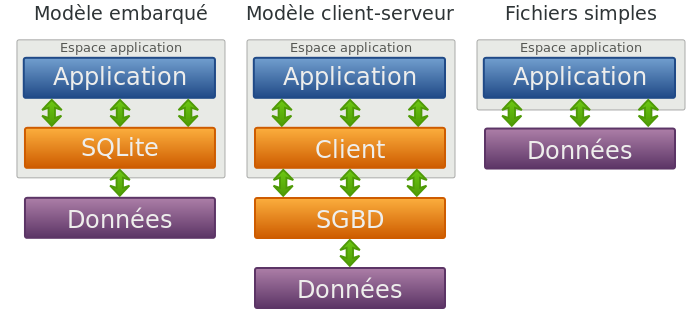
\includegraphics[width=10cm]{ressources/modeles.png}
        \captionof{figure}{Modèles d'accès aux données}
        \label{IMG}
    \end{center}

\end{frame}
\subsection{Retour historique}
\begin{frame}
    \frametitle{Retour historique}

    \begin{center}
        \centering
        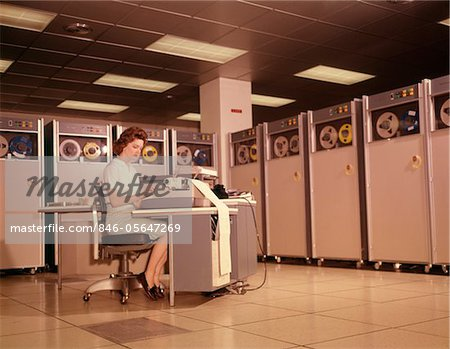
\includegraphics[width=8cm]{ressources/bande.jpg}
        \captionof{figure}{\centering avant 1960: données sur bandes magnétiques}
        \label{IMG}
    \end{center}
    \begin{aretenir}[Remarque]
        L'arrivée des stockages à accès direct change la manière de traiter les données.
    \end{aretenir}
\end{frame}
\begin{frame}

    \begin{center}
        \centering
        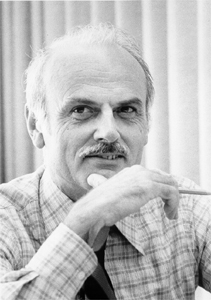
\includegraphics[width=5cm]{ressources/codd.jpg}
        \captionof{figure}{\centering 1970: Edgar Codd propose le \emph{modèle relationnel}}
        \label{IMG}
    \end{center}
    \note{remplace modèle hiérarchique}
\end{frame}
\begin{frame}

    \begin{center}
        \centering
        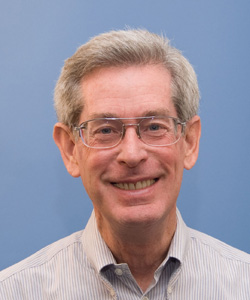
\includegraphics[width=5cm]{ressources/chamberlin.jpg}
        \captionof{figure}{\centering 1974: Donald Chamberlin développe le langage \textbf{SQL} pour communiquer avec les bases de données}
        \label{IMG}
    \end{center}
    \note{normalisé en 1986 par ISO (International Organization for Standardization)}
\end{frame}
\begin{frame}

    \begin{center}
        \centering
        
\includegraphics[width=4cm]{ressources/oracle.png}
        \captionof{figure}{\centering fin 70: Oracle (système propriétaire)}
        \label{IMG}
    \end{center}
    \note{au début pour missiles embarqués}
\end{frame}
\begin{frame}

    \begin{center}
        \centering
        
\includegraphics[width=4cm]{ressources/postgresql.png}
        \captionof{figure}{\centering 1985: PostgreSQL (logiciel libre fondé sur une communauté mondiale de développeurs)}
        \label{IMG}
    \end{center}
\end{frame}

\begin{frame}

    \begin{center}
        \centering
        
\includegraphics[width=4cm]{ressources/mysql.png}
        \captionof{figure}{\centering 1995: Mickael Winedius développe MySQL (Licence GNU - General Public License)}
        \label{IMG}
    \end{center}
    \note{le + utilisé}
\end{frame}
\begin{frame}

    \begin{center}
        \centering
        
\includegraphics[width=4cm]{ressources/sqlite.png}
        \captionof{figure}{\centering 2000: Sqlite (n'utilise pas de système client-serveur)}
        \label{IMG}
    \end{center}
    \note{au début pour missiles embarqués}
\end{frame}
\begin{frame}

    \begin{center}
        \centering
        
\includegraphics[width=4cm]{ressources/maria.png}
        \captionof{figure}{\centering 2009: Winedius développe MariaDB suite au rachat de MySQL par Sun puis Oracle}
        \label{IMG}
    \end{center}
    \note{le + utilisé}
\end{frame}
\subsection{Un langage}
\begin{frame}
    \frametitle{Un langage}

    Les SGBD stockent et optimisent les données de manière efficace mais très complexe. Il n'est pas possible d'y accéder directement. Il faut effectuer des \textbf{requêtes} à l'aide d'un langage adapté.

\end{frame}
\begin{frame}
    \frametitle{}

    \begin{aretenir}[]
        Le \textbf{SQL (Structured Query Language)} est utilisé dans une écrasante majorité des SGBDR.
    \end{aretenir}
    \note{concurrents: QBE (Query By Example) utilisé dans Microsoft Access	(SGBDR de type "fichier")\\
        modèle "fichier simple": traitement de texte; .doc, .odt = xml empaqueté }
\end{frame}
\begin{frame}
    \frametitle{}

    \begin{center}
        \centering
        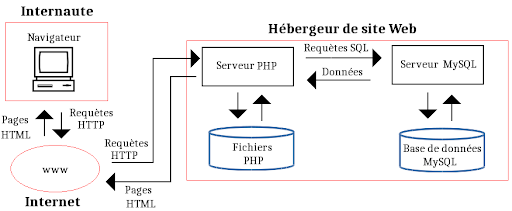
\includegraphics[width=10cm]{ressources/requete-http.png}
        \captionof{figure}{Répartition des rôles}
        \label{IMG}
    \end{center}

\end{frame}
\section{Contraintes d'intégrité}
\subsection{Ouvrir un SGBD}
\begin{frame}
    \frametitle{Contraintes d'intégrité - Ouvrir un SGBD}

    \begin{activite}
        \begin{enumerate}
            \item Télécharger et extraire la version portable de \emph{DB Browser for SQLite} depuis le site officiel \mbox{\url{https://sqlitebrowser.org/dl/}}
            \item Télécharger et extraire la base \emph{bd-initialisation.zip} depuis le site \mbox{\url{https://cviroulaud.github.io}}
            \item Ouvrir la base avec le browser.
            \item Se concentrer d'abord sur l'onglet \emph{Parcourir les données} et observer les tables existantes.
        \end{enumerate}
    \end{activite}

\end{frame}
\subsection{Contrainte de domaine}
\begin{frame}
    \frametitle{Contrainte de domaine}

    Aux domaines abstraits du modèle relationnel correspondent les types de données du langage SQL.
\begin{center}
\begin{tabular}{|c|c|}
\hline 
\textbf{Nom du type} & \textbf{Description} \\ 
\hline 
SMALLINT & Entier 16 bits signé \\ 
\hline 
INT & Entier 32 bits signé \\ 
\hline 
BIGINT & Entier 64 bit signé \\ 
\hline 
REAL & Flottant 32 bits \\ 
\hline 
CHAR(n) & Chaîne de n caractères exactement \\ 
\hline 
VARCHAR(n) & Chaîne d'au plus n caractères \\ 
\hline 
TEXT & Chaîne de taille quelconque \\ 
\hline 
DATE & Date au format AAAA-MM-JJ \\ 
\hline 
TIME & Heure au format hh:mm:ss \\ 
\hline 
TIMESTAMP & Instant au format AAAA-MM-JJ hh:mm:ss \\ 
\hline 
\end{tabular}
\end{center}
\note[item]{TINYINT 1 octet}
\note[item]{BOOLEAN garantit que 2 valeurs; mais pas également supporté}
\end{frame}
\begin{frame}
    \frametitle{}
\begin{activite}
    \begin{enumerate}
        \item Quelle est la valeur maximale que peut prendre un \textbf{SMALLINT}?
        \item Quelle sa taille en mémoire?
        \item Dans le browser, se rendre dans l'onglet \emph{Structure de la base de données}.
        \item Dérouler la table \texttt{\textbf{Auteurs}} et repérer les types de chaque attribut.
        \end{enumerate}
        \end{activite}

\end{frame}
\begin{frame}
    \frametitle{}

    SMALLINT sur 2 octets donc:
    \begin{itemize}
        \item le maximum est $2^{16}-1$
        \item ou $2^{15}-1$ si l'entier est signé
    \end{itemize}
\begin{aretenir}[Remarque]
    Le SGBD Sqlite simplifie les types (INTEGER, REAL, TEXT) en l'adaptant dynamiquement en fonction de la valeur stockée.
\end{aretenir}
\end{frame}
\subsection{Contrainte d'entité}
\begin{frame}
    \frametitle{Contrainte d'entité}

    Chaque entité est identifiée de manière unique grâce à la \emph{clé primaire}.
    \begin{activite}
    \begin{enumerate}
    \item Dans le schéma de la table \texttt{\textbf{Auteurs}} comment identifie-t-on la clé primaire?
    \item Quel est le rôle du mot clé \texttt{\textbf{AUTOINCREMENT}}?
    \end{enumerate}
    \end{activite}

\end{frame}
\begin{frame}
    \frametitle{Correction}

    \begin{itemize}
        \item clé primaire: \texttt{\textbf{PRIMARY KEY}}
        \item \texttt{\textbf{AUTOINCREMENT:}} augmentation automatique de l'identifiant à la création d'une nouvelle identité
    \end{itemize}

\end{frame}
\subsection{Contrainte de référence}
\begin{frame}
    \frametitle{Contrainte de référence}

    Afin de garantir la cohérence des données lors de modifications, on utilise une \emph{clé étrangère}. C'est une référence à une clé primaire d'une autre relation.
\begin{activite}
\begin{enumerate}
\item Dérouler la table \texttt{\textbf{Bandes\_dessinees}}.
\item Rappeler les attributs qui sont des clés étrangères.
\item Glisser la souris sur le schéma de cette table. Quels mots clés sont utilisés pour créer une clé étrangère?
\end{enumerate}
\end{activite}

\end{frame}
\begin{frame}
    \frametitle{Correction}

    clé étrangère: \textbf{FOREIGN KEY(id\_genre) REFERENCES Genres.id}

\end{frame}
\subsection{Compléter la base de données}
\begin{frame}
    \frametitle{Compléter la base de données}

    \begin{activite}
        Depuis l'onglet \emph{Exécuter le SQL}, créer les tables \textbf{Emprunteurs} et \textbf{Emprunts}, en prenant modèle sur les schémas des relations existantes.
        \end{activite}
        \begin{aretenir}[Remarque]
        Le langage SQL est insensible à la casse. Nous pouvons écrire indifféremment \emph{CREATE} ou \emph{CreaTE}. Il est d'usage d'écrire les instructions SQL en majuscules.
        \end{aretenir}    

\end{frame}
\begin{frame}[fragile]
    \frametitle{Correction}

    \begin{center}
    \begin{lstlisting}[language=sql , basicstyle=\ttfamily\small, xleftmargin=1em, xrightmargin=-1em]
CREATE TABLE Emprunteurs( id INTEGER PRIMARY KEY AUTOINCREMENT, 
prenom TEXT, 
nom TEXT, 
naissance TEXT);

CREATE TABLE Emprunts( isbn INTEGER PRIMARY KEY,
id_emprunteurs INTEGER, 
FOREIGN KEY (isbn) REFERENCES Bandes_dessinees(isbn), 
FOREIGN KEY (id_emprunteurs) REFERENCES Emprunteurs(id) );
\end{lstlisting}
    \end{center}

\end{frame}
\end{document}